\chapter{Introduction}
\label{cha:intro}

This chapter highlights the aims and objectives of this project, and how it may impact on the improvement of an ongoing research XXXX worth lots... lol

\section{Background}
\label{sec:background}

"SpiNNaker is a biologically inspired, massively parallel computing engine designed to facilitate the modelling and simulation of large-scale spiking neural networks of up to a billion neurons and trillion synapses (inter-neuron connections) in biological real time."\cite{painkras} Spinnaker was designed at the University of Manchester within an EPSRC-funded project in collaboration with other institutions.XXX

The Spinnaker research, funded by the Human Brain Project (HBP)[definition] started on XXX 2005? XXX and has the XX final aim? XX of simulating the human brain.

A standard Spinnaker board is composed of 48 descentralised, power efficient, Spinnaker chip multiprocessor (CMP) dies, each containing 18 ARM968 processing cores sharing 128-MB of in-chip dynamic memory (SDRAM). In a standard environment each ARM models up to 1000 neurons, which can communicate to each other through atomic 'spike' events using the on- and inter-chip communication fabric.\cite{datasheet}

event driven architecture

\begin{figure}
\begin{center}
	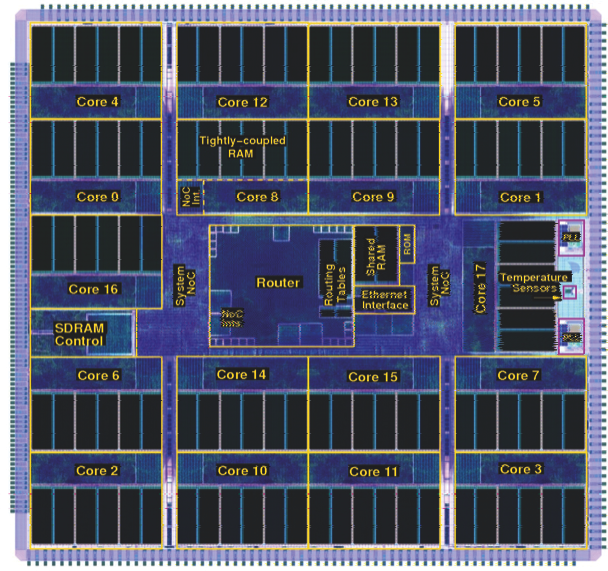
\includegraphics[width=1\textwidth, natwidth=608, natheight=571]{images/chip.png}
\end{center}
\caption{SpiNNaker chip layout}
\end{figure}

\section{Project Aim}
\label{sec:aim}

This research project involves making use of the emerging SpiNNaker software stack and hardware infrastructure, both optimised for neural network simulations, in order to explore and evaluate its usability and performance as a general purpose platform. This has been achieved through the development of a distributed Key-Value store and a Relational Database Management System with limited scope.

In addition to usability testing, performance benchmarks have been gathered for this application, allowing analysis which can provide insights for improvements to the current architecture, possibly influencing on changes to reflect on the next generation of the chip: SpiNNaker 2. A 

aim: balance of memory and processing power on the chip, etc.
